\documentclass[12pt]{article}
\usepackage[a4paper]{geometry}
\usepackage[pdftex]{hyperref}
\usepackage[german]{babel}
\usepackage[utf8]{inputenc}
\usepackage{csquotes}
\usepackage{amssymb}
\usepackage{graphicx}
\usepackage{multicol}
\usepackage{amsmath}
\usepackage{enumitem}
\usepackage{fancyhdr}
\usepackage{indentfirst}
\usepackage{polynom}

\geometry{
  headheight=14px,
  left=2.54cm,
  right=2.54cm,
  bottom=2cm,
  top=2cm
}

\setlength{\marginparsep}{1 cm}
\setlength{\topmargin}{-0.6in}
\setlength{\textheight}{9.5in}
\pagestyle{fancy}

% German-style quotation marks %
\MakeOuterQuote{"}

% Typesetting differential operator %
\providecommand\d{}
\renewcommand{\d}[1]{\:\mathrm{d}{#1}} 

\polyset{%
   style=C,
   delims={\big(}{\big)},
   div=:
}

\fancypagestyle{firstpage}{%
  \lhead{\bf Name:}
  \rhead{\bf Anzahl zusätzlicher Blätter:\space\space\space\space\space}
}

\begin{document}

\thispagestyle{firstpage}

\begin{center}
{\bf {\large Klausur Analysis (3IT18-1, 3MI18-1) - 27.02.2019}}
\end{center}

\begin{center}
\textbf {Der Rechengang muss eindeutig und vollständig ersichtlich sein!}
\end{center}

\textbf{Hilfsmittel}: Kein Taschenrechner, ein handbeschriebenes A4-Blatt.

\begin{center}
Bitte nutzen Sie nach Möglichkeit den Platz auf den Aufgabenblättern und den Rückseiten. Zusätzlich beschriebene Blätter heften Sie bitte an diese Klausur.
\end{center}

\section*{Bewertung}

\begin{itemize}
\item Aufgabe 1:      \space\space\space\space\space$/12$
\item Aufgabe 2:      \space\space\space\space\space$/07$
\item Aufgabe 3:      \space\space\space\space\space$/10$
\item Aufgabe 4:      \space\space\space\space\space$/13$
\item Zusatzaufgabe:  \space\space\space\space\space$/02$
\end{itemize}

\textbf{Gesamt}: \space\space\space\space\space %$/$

\textbf{Note}:

\begin{center}
{\bf {\large Viel Erfolg!}}
\end{center}


%\begin{center}
%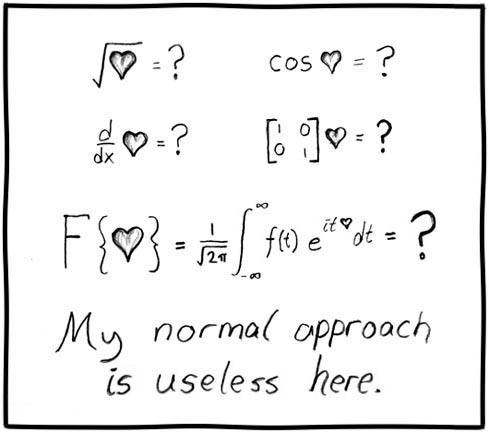
\includegraphics[width=0.4\textwidth]{useless.jpg}
%https://xkcd.com/55/
%\end{center}

\newpage
\section* {Aufgabe 1}

Gegeben sei die Funktion $f(x) = \cos(0{,}5 \pi x + \pi)$.

\begin{enumerate}[label=(\alph*)]
\item (3P) Die Funktion $f$ entsteht aus der Funktion $g(x) = \cos(x)$ durch Verschiebung und Skalierung. Um wie viel und entlang welcher Achse wird verschoben und skaliert?
\item (3P) Skizzieren Sie die Funktion $f$!
\item (4P) Skizzieren Sie die graphische Bedeutung der Ausdrücke $f'(0)$ und $\int_0^2 f(x)\d x$! Lesen Sie die Werte dieser beiden Ausdrücke aus der Skizze ab!
\item (2P) Durch $M_{n}[f] := \sum\limits_{k=0}^n \frac{f^{(k)}(0)}{k!}x^k$ ist die Maclaurin-Reihe der Funktion $f(x)$ gegeben. Welche graphische Bedeutung haben $M_1[f]$ und $M_2[f]$?
\end {enumerate}

\begin{center}
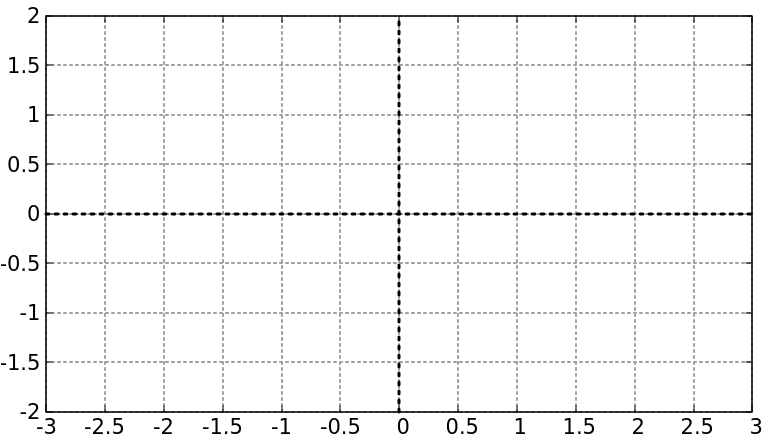
\includegraphics[width=0.8\textwidth]{grid_klausur.png}
\end{center}

\newpage
\section* {Aufgabe 2}

Eine Funktion $f(x)$ heißt punktsymmetrisch bzgl. des Punktes $(x_0,y_0) \in\mathbb{R}^2$, falls folgende Bedingung erfüllt ist:

$$\forall x \in \mathbb{R}: f(x_0-x)+f(x_0+x)=2y_0$$ 

\begin{enumerate}[label=(\alph*)]

\item (4P) Untersuchen Sie anhand dieser Bedingung, ob $f(x) = \sin(2x-2)+1$ punktsymmetrisch ist bezüglich des Punkts $(1,1)$! (Hinweis: $\sin(-x)=-\sin(x)$)

\item  (3P) Es soll untersucht werden, zu welchem Punkt $(x_0,y_0)$ die Funktion \\
$f(x) = x^3-3x^2+3x$ punktsymmetrisch ist. Die Auswertung der Bedingung ergab:

$$(6x_0-6) x^2 + 2x_0^3 - 6x_0^2 + 6x_0 = 2y_0$$

Welchen Wert hat ($x_0,y_0)$? (Hinweis: Koeffizientenvergleich.)

\end{enumerate}

\newpage
\section* {Aufgabe 3}

Es soll die folgende zweistellige Funktion betrachtet werden:

$$f(x,y)=\frac{x^3+x^2y-xy^2-y^3}{x-y}$$

Durch Termumformung (für $x \neq y$) kann man zeigen:

$$f(x,y) = x^2+2xy+y^2$$

\begin{enumerate}[label=(\alph*)]
\item (3P) Beweisen Sie, dass die Termumformung korrekt ist, indem Sie eine Polynomdivision durchführen! (Hinweis: Betrachten Sie $y$ als Konstante.)

\polylongdiv[stage=1]{x^3+yx^2-y^2x-y^3}{x-y}

\bigskip
\bigskip
\bigskip
\bigskip
\bigskip
\bigskip
\bigskip
\bigskip
\bigskip
\bigskip
\bigskip
\bigskip
\bigskip
\bigskip
\bigskip

\item (5P) Berechnen Sie die partiellen Ableitungen $f_x$, $f_y$ und $f_{xy}$ und $f_{yx}$! Stimmt hier der Satz von Schwarz?

\item (2P) Welche notwendige Bedingung muss gelten, damit $f$ in $(x_0,y_0)$ eine lokale Extremstelle besitzen kann? Welche Punkte $(x_0,y_0)$ kommen daher in Betracht für die Funktion $f(x,y)$?

\end{enumerate}

\newpage
\section* {Aufgabe 4}

Gesucht ist die allgemeine Lösung der Differentialgleichung (DGL)

$$y'=y\frac{2x}{x^2+1}$$

\begin{enumerate}[label=(\alph*)]
\item (6P) Klassifizieren Sie diese DGL bezüglich Ordnung, Homogenität, Linearität. (Begründung!)
\item (3P) Sie kann mittels der Methode "Trennung der Variablen" gelöst werden. Finden Sie die beiden Integrale, die dabei zu lösen wären!
\item (4P) Lösen Sie das Integral über $x$, indem Sie die Substitution $u=x^2+1$ anwenden.
\end{enumerate}

\newpage
\section*{Zusatzaufgabe (2P)}


In der klassischen Mechanik beschreibt die Lagrange-Funktion $L(x,\dot x, t) = E_{kin} - E_{pot}$ ein mechanisches System. Für ein Federpendel lautet die Lagrange-Funktion $L=\frac{m}{2}\dot{x}^2 - \frac{k}{2}x^2$. Das sogenannte "Noether-Theorem" stellt einen Zusammenhang her zwischen Symmetrien und Erhaltungsgrößen. Sind die Bewegungsgleichungen invariant unter einer Koordinatentransformation $t \to t+\Delta t\cdot\gamma$, so ist die Größe $Q=\left(\dot x \cdot \frac{\partial L}{\partial \dot x} - L\right)\cdot\gamma$ eine Erhaltungsgröße. Das Pendel schwingt immer gleichartig, egal, wann man es anstößt, d.h. $\gamma = 1$. Wie lautet die zugehörige Erhaltungsgröße $Q$ für das Pendel? Was ist das für eine physikalische Größe?

\newpage

\begin{center}
{\bf {\large Musterlösung}}
\end{center}

\begin{center}
{\bf {\large Klausur Analysis (3IT18-1, 3MI18-1) - 27.02.2019}}
\end{center}

\begin{center}
\textbf{Jeder Anführungspunkt entspricht einem erteilten Bewertungspunkt.}
\end{center}

Pro Aufgabe gibt es einen Punkt Abzug, falls formal inkorrekte Schreibweisen verwendet werden. Beispiel: 
$$f(x)=\sin(x), f'(x)=\cos(x)=0$$

Mit dem letzten Gleichheitszeichen ist eigentlich gemeint, dass $f'(0)$  berechnet wurde.

\begin{enumerate}

% Task 1
\item
\begin{enumerate}
\item $f(x) = \cos(0,5\pi x+\pi) = \cos(0,5\pi(x+2))$
\begin{itemize}
\item Verschiebung entlang x-Achse, Skalierung entlang x-Achse
\item 2 Einheiten nach links
\item mit dem Faktor $0,5\pi$
\end{itemize}

\item Der Graph muss aussehen wie eine Kosinusfunktion, die wie in $(a)$ beschrieben verschoben ist:
\begin{itemize}
\item Amplitude ist korrekt eingetragen (von -1 bis +1)
\item Verschiebung ist korrekt eingetragen (2 nach links)
\item Periode ist korrekt eingetragen ($\frac{2\pi}{\frac{\pi}{2}} = 4$)
\end{itemize}

\begin{figure}[ht]
	\centering
	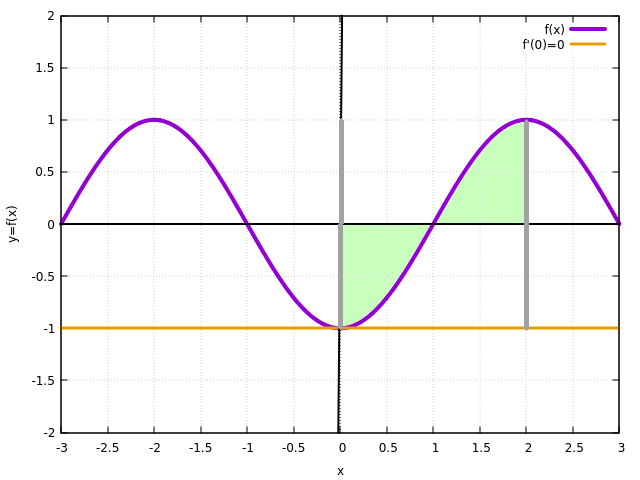
\includegraphics[width=0.4\textwidth]{grid_klausur_lsg.png}
	\caption{Skizze zu Aufgabe 1. Grün markiert ist der gerichtete Flächeninhalt zwischen $0\le x \le 2$.}
	\label{fig1}
\end{figure}


\item 
\begin{itemize}
\item $f'(0)$ ist Tangente bei $x=0$
\item $f'(0) = 0$
\item $\int_0^2 f(x) \d x$ ist (vorzeichenbehaftete) Fläche zwischen Graph und x-Achse zwischen 0 und 2
\item $\int_0^2 f(x) \d x = 0$
\end{itemize}

\item
\begin{itemize}
\item Tangente und (Schmiege-)parabel
\item An der Stelle $x_0=0$
\end{itemize}

\end{enumerate}

% Task 2
\item
\begin{enumerate}

\item 
\begin{itemize}
\item $x_0=1, y_0=1$
\item $f(1-x) = \sin(2-2x-2)+1=-\sin(2x) + 1$
\item $f(1+x) = \sin(2+2x-2)+1=\sin(2x) + 1$
\item Somit $f(1-x)+f(1+x)=2$, also punktsymmetrisch bzgl. $(1,1)$
\end{itemize}

\item 
\begin{itemize}
\item $6x_0-6=0$, also $x_0=1$.
\item $[2x_0^3-6x_0^2+6x_0]_{x_0=1}=2-6+6=2=2y_0$
\item Also $y_0 = 1$.
\end{itemize}

\end{enumerate}

% Task 3

\item
\begin{enumerate}

\item
\[\polylongdiv{x^3+yx^2-y^2x-y^3}{x-y}\]
\begin{itemize}
\item Für den ersten Schritt der Polynomdivision
\item Für den zweiten Schritt der Polynomdivision
\item Für den dritten Schritt der Polynomdivision und das Ergebnis
\end{itemize}

\item 
\begin{itemize}
\item $f_x = 2x+2y$
\item $f_y = 2y+2x$
\item $f_{xy} = 2$
\item $f_{yx} = 2$
\item $f_{xy} = f_{yx}$, also stimmt Satz von Schwarz hier. Falls falsches Ergebnis für die Ableitungen berechnet wurde, wobei $f_{xy} \neq f_{yx}$, so nur Punkt, falls folgerichtig gesagt wird, der Satz von Schwarz stimme nicht.
\end{itemize}

\item 
\begin{itemize}
\item $f_x(x_0,y_0) = f_y(x_0,y_0) = 0$
\item $2x_0+2y_0=0$, also die Punkte $(t,-t), t \in \mathbb{R}$ 
\end{itemize}

\end{enumerate}

% Task 4

\item
\begin{enumerate}

\item $(x^2+1)\cdot y'-2x\cdot y = 0$
\begin{itemize}
\item Ordnung 1
\item Weil $y'$ höchste Ableitung
\item Homogen
\item Weil $(x^2+1)\cdot(ty)'-2x\cdot(ty) = t^1 ((x^2+1)\cdot y'-2x\cdot y)$
\item Linear
\item Weil Grad der Homogenität gleich 1
\end{itemize}

\item 
\begin{itemize}
\item $\frac{\d y}{\d x} = y \frac{2x}{x^2+1}$
\item $\implies \frac{\d y}{y} = \frac{2x}{x^2+1}\d x$
\item $\implies \int \frac{\d y}{y} = \int \frac{2x}{x^2+1}\d x$
\end{itemize}

\item Der Betrag im letzten Schritt fällt weg, da $x^2+1>0$ für alle $x \in \mathbb{R}$ gilt.
\begin{itemize}
\item $u=x^2+1, \d u = 2x \d x$ (Ableiten der Substitution)
\item $\int \frac{2x}{x^2+1}\d x = \int \frac{2x\d u}{u\cdot 2x}$
\item $= \int \frac{\d u}{u} = \ln(|u|)+C$ (Konstante)
\item $= \ln(x^2+1)+C$ (Rücksubstitution)
\end{itemize}

\end{enumerate}

\end{enumerate}

\subsection*{Zusatzaufgabe}

\begin{itemize}
\item $\frac{\partial L}{\partial \dot x} = \frac{\partial L}{\partial \dot x} \left(\frac{m}{2}\dot{x}^2 - \frac{k}{2}x^2\right) = m\dot x$
\item Die Größe $Q=(\dot x \cdot m\dot x - \frac{m}{2}\dot x^2 + \frac{k}{2}x^2)\cdot 1 = \frac{m}{2}\dot x^2 + \frac{k}{2}x^2 = E_{kin}+E_{pot}$ ist die Gesamtenergie, es gilt also Energieerhaltung.
\end{itemize}


\end{document}
